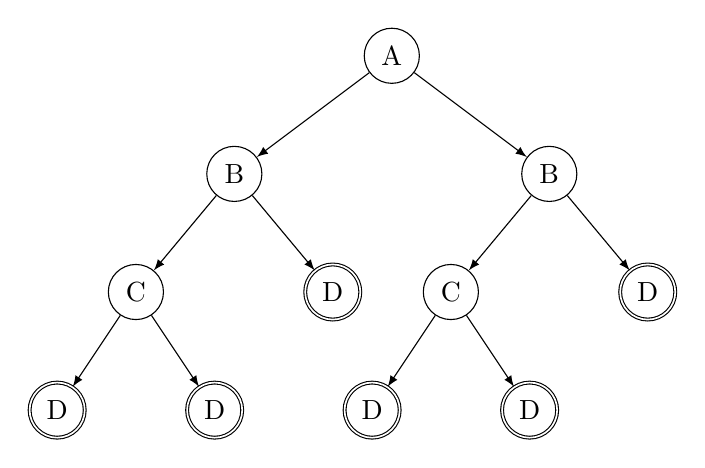
\begin{tikzpicture}[
    level distance=1.5cm,
    sibling distance=3cm,
    state/.style={circle, draw, minimum size=7mm},
    accepting/.style={circle, draw, double, minimum size=7mm},
    edge from parent/.style={draw, -latex},
    level 1/.style={sibling distance=4cm},
    level 2/.style={sibling distance=2.5cm},
    level 3/.style={sibling distance=2cm}
    ]

\node[state] (a) {A}
    child {node[state] (b) {B} 
    child {node[state] (d) {C}
        child {node[accepting] (h) {D}}
        child {node[accepting] (i) {D}}
    }
    child {node[accepting] (e) {D}}
    }
    child {node[state] (c) {B}
    child {node[state] (f) {C}
        child {node[accepting] (l) {D}}
        child {node[accepting] (m) {D}}
    }
    child {node[accepting] (g) {D}}
    };
\end{tikzpicture}